\chapter{The Monte Carlo Random Walk Process for Adjoint Radiation Transport}
\label{ch:adjoint_particle_transport}
In chapter \ref{ch:mc_methods}, the dual problem for calculating inner products
over small phase spaces was introduced. In this chapter, it will be shown how
the dual problem can be solved in the context of radiation transport 
problems. This will require both the derivation of the dual problems of interest
and their associated Monte Carlo random walk processes. Since, in the previous
chapter, the FEISKs that described the event densities were shown to have 
ideal random walk PDFs, their dual problems will be evaluated first. The 
random walk process for the more general dual problem, which is characterized
by the adjoint transport equation, will then be determined. 

\section{The Adjoint of the Emission Density FIESK}
Using the procedure outlined in chapter \ref{ch:mc_methods}, the dual emission
density FIESK will be constructed. The function that will solve this dual 
equation will be called the adjoint of the emission density. It is not called
the adjoint emission density because, as will be shown, this function does
not behave like an emission density (or in general an event density). First, 
a linear operator will be constructed from equation 
\ref{eq:emission_density_integral_eqn}, which is the emission density FIESK. 
\begin{equation}
  \begin{split}
    H_{\chi} \cdot &\chi(\vec{r},E,\hat{\Omega}) = 
    \chi(\vec{r},E,\hat{\Omega}) - \\
    & \int\int\int C(\vec{r},E^{'} \to E,\hat{\Omega}^{'} \to \hat{\Omega})
    T(\vec{r}^{'} \to \vec{r},E^{'},\hat{\Omega}^{'}) 
    \chi(\vec{r}^{'},E',\hat{\Omega}^{'}) dV^{'}dE^{'}E\hat{\Omega}^{'}
  \end{split}
\end{equation}
With the operator $H_{\chi}$ defined in this way it is clear from equation
\ref{eq:emission_density_integral_eqn} that 
$H_{\chi} = S(\vec{r},E,\hat{\Omega})$.

To define the adjoint operator, the following equality must hold. Where the 
brackets indicate integration over all phase space.
\begin{equation*}
  \langle \chi^{\dagger}H_{\chi} \cdot \chi \rangle = 
  \langle \chi H_{\chi}^{\dagger} \cdot \chi^{\dagger} \rangle
\end{equation*}
Since the operator $H_{\chi}$ is known, the left bracket will be expanded.
\begin{align}
  \langle \chi^{\dagger}H_{\chi} \cdot \chi \rangle & =
  \int\int\int \
  \chi^{\dagger}(\vec{r},E,\hat{\Omega}) \chi(\vec{r},E,\hat{\Omega})
  dV dE d\hat{\Omega} - \int\int\int \chi^{\dagger}(\vec{r},E,\hat{\Omega}) 
  \nonumber \\
  \cdot \int\int\int 
  C(\vec{r}&,E^{'} \to E, \hat{\Omega}^{'} \to \hat{\Omega}^{'})
  T(\vec{r}^{'} \to \vec{r},E^{'},\hat{\Omega}^{'})
  \chi(\vec{r}^{'},E^{'},\hat{\Omega}^{'}) dV^{'}dE^{'}d\hat{\Omega}^{'}
  dV dE d\hat{\Omega} \nonumber \\
  & = \int\int\int \
  \chi^{\dagger}(\vec{r},E,\hat{\Omega}) \chi(\vec{r},E,\hat{\Omega})
  dV dE d\hat{\Omega} - \int\int\int \chi(\vec{r}^{'},E^{'},\hat{\Omega}^{'}) 
  \nonumber \\
  \cdot \int\int\int 
  C(\vec{r}&,E^{'} \to E, \hat{\Omega}^{'} \to \hat{\Omega}^{'})
  T(\vec{r}^{'} \to \vec{r},E^{'},\hat{\Omega}^{'})
  \chi^{\dagger}(\vec{r},E,\hat{\Omega}) dV dE d\hat{\Omega}
  dV^{'}dE^{'}d\hat{\Omega}^{'}
\end{align}
From this last manipulation, the adjoint operator can be deduced, which is 
shown in the following equation.
\begin{equation}
  \begin{split}
    H_{\chi}^{\dagger} \cdot &\chi^{\dagger}(\vec{r},E,\hat{\Omega}) = 
    \chi^{\dagger}(\vec{r},E,\hat{\Omega}) - \\
    & \int\int\int T(\vec{r} \to \vec{r}^{'},E,\hat{\Omega}) 
    C(\vec{r}^{'},E \to E^{'},\hat{\Omega} \to \hat{\Omega}^{'})
    \chi(\vec{r}^{'},E',\hat{\Omega}^{'}) dE^{'}d\hat{\Omega}^{'}dV^{'}
  \end{split}
\end{equation}

In the previous chapter, the function $c(\vec{r},E,\hat{\Omega})$ was defined 
in equation \ref{eq:emission_response_function}, which should be used with 
the emission density to calculate a response. By forcing the adjoint 
operator acting on the adjoint of the emission density to equal the 
function $c(\vec{r},E,\hat{\Omega})$, the dual equation, or simply the adjoint
of the emission density FIESK can be created.
\begin{equation}
  \begin{split}
    \chi^{\dagger}(\vec{r},&E,\hat{\Omega}) = c(\vec{r},E,\hat{\Omega}) + \\
    &\int\int\int T(\vec{r} \to \vec{r}^{'},E,\hat{\Omega}) 
    C(\vec{r}^{'},E \to E^{'},\hat{\Omega} \to \hat{\Omega}^{'})
    \chi^{\dagger}(\vec{r}^{'},E',\hat{\Omega}^{'}) dE^{'}d\hat{\Omega}^{'}dV^{'}
  \end{split}
  \label{eq:adjoint_of_emission_density_integral_eqn}
\end{equation}

Unfortunately, in the integral in equation 
\ref{eq:adjoint_of_emission_density_integral_eqn}, the transport and collision 
kernels are integrated over what was previously the final states. Therefore,
the properties that were defined for these kernels in the previous chapter are 
no longer valid. In particular, the transport kernel is not normalized anymore
and the collision kernel is not equal to the average number of particles 
emitted from a collision when integrated over all final states. To try and 
simplify these kernels, the $\Sigma_T(\vec{r}^{'},E)$ terms  in both the 
transport and collision kernels will be allowed to cancel each other out. The 
modified transport kernel will now be examined.
\begin{equation}
  \frac{T(\vec{r} \to \vec{r}^{'},E,\hat{\Omega})}{\Sigma_T(\vec{r}^{'},E)} = 
  exp\left[-\int_0^{|\vec{r}^{'} - \vec{r}|} 
    \Sigma_T(\vec{r}^{'} - R^{'} \hat{\Omega},E)dR^{'} \right]
  \frac{\delta \left(\Omega - \left[\frac{\vec{r}^{'} - \vec{r}}
      {|\vec{r}^{'} - \vec{r}|}\right]\right)}
       {|\vec{r}^{'} - \vec{r}|^2}
  \label{eq:unnormalized_adjoint_transport_kernel}
\end{equation}
Based on the argument of the delta function, 
$\hat{\Omega} = \frac{\vec{r}^{'} - \vec{r}}{|\vec{r}^{'} - \vec{r}|}$ and 
therefore, $\vec{r}^{'} = \vec{r} + \hat{\Omega}|\vec{r}^{'} - \vec{r}|$. This
equation for $\vec{r}^{'}$ can be substituted back into the equation
\ref{eq:unnormalized_adjoint_transport_kernel}.
\begin{equation*}
  \frac{T(\vec{r} \to \vec{r}^{'},E,\hat{\Omega})}{\Sigma_T(\vec{r}^{'},E)} = 
  exp\left[-\int_0^{|\vec{r}^{'} - \vec{r}|} 
    \Sigma_T \left(\vec{r} + \left[|\vec{r}^{'} - \vec{r}| - R^{'} \right] 
    \hat{\Omega},E \right) dR^{'} 
    \right] \frac{\delta \left(\Omega - \left[\frac{\vec{r}^{'} - \vec{r}}
      {|\vec{r}^{'} - \vec{r}|}\right]\right)}
       {|\vec{r}^{'} - \vec{r}|^2}
\end{equation*}
A new variable of integration can be defined to simplify the exponent. Note
that when $R^{'} = 0$, $R^{''} = |\vec{r}^{'} - \vec{r}|$ and when 
$R^{'} = |\vec{r}^{'} - \vec{r}|$, $R^{''} = 0$.
\begin{align}
  R^{''} & = |\vec{r}^{'} - \vec{r}| - R^{'} \nonumber \\
  dR^{''} & = -dR^{'} \nonumber 
\end{align}
\begin{align}
  \frac{T(\vec{r} \to \vec{r}^{'},E,\hat{\Omega})}{\Sigma_T(\vec{r}^{'},E)} & =
  exp\left[-\int_0^{|\vec{r}^{'} - \vec{r}|} 
    \Sigma_T \left(\vec{r} + R^{''}\hat{\Omega},E \right) dR^{''} 
    \right] \frac{\delta \left(\Omega - \left[\frac{\vec{r}^{'} - \vec{r}}
      {|\vec{r}^{'} - \vec{r}|}\right]\right)}
       {|\vec{r}^{'} - \vec{r}|^2} \nonumber \\
       & = exp\left[-\int_0^{|\vec{r} - \vec{r}^{'}|} 
    \Sigma_T \left(\vec{r} + R^{''}\hat{\Omega},E \right) dR^{''} 
    \right] \frac{\delta \left(\Omega + \left[\frac{\vec{r} - \vec{r}^{'}}
      {|\vec{r} - \vec{r}^{'}|}\right]\right)}
       {|\vec{r} - \vec{r}^{'}|^2} \nonumber \\
       & = \tau(\vec{r}^{'},\vec{r},E,-\hat{\Omega}) \\
       & = \frac{T(\vec{r}^{'} \to \vec{r},E,-\hat{\Omega})}
       {\Sigma_T(\vec{r},E)}
\end{align}
The complete adjoint of the emission density state transition kernel can now be 
defined.
\begin{equation}
  K^{\dagger}(\vec{r}^{'} \to \vec{r},E^{'} \to E,
  \hat{\Omega}^{'} \to \hat{\Omega}) = 
  \tau(\vec{r}^{'},\vec{r},E,-\hat{\Omega}) 
  \Sigma_T(\vec{r}^{'},E \to E^{'},\hat{\Omega} \to \hat{\Omega}^{'})
\end{equation}
The source term $c(\vec{r},E,\hat{\Omega})$ can also be modified, since it
contains the modified transport kernel.
\begin{align}
  c(\vec{r},E,\hat{\Omega}) & = \int \frac{a(\vec{r}^{'},E,\hat{\Omega})}
  {\Sigma_T(\vec{r}^{'},E)}T(\vec{r} \to \vec{r}^{'},E,\hat{\Omega}) dV^{'} 
  \nonumber \\
  & = \int a(\vec{r}^{'},E,\hat{\Omega}) 
  \tau(\vec{r}^{'},\vec{r},E,-\hat{\Omega}) dV^{'}
\end{align}
Finally, the adjoint of the emission density FIESK can be rewritten with the 
modifications that were just described.
\begin{equation}
  \begin{split}
    \chi^{\dagger}(\vec{r},E,\hat{\Omega}) =  \int a(\vec{r}^{'},&E,\hat{\Omega}) 
    \tau(\vec{r}^{'},\vec{r},E,-\hat{\Omega}) dV^{'} + \\
    & \int\int\int  \tau(\vec{r}^{'},\vec{r},E,-\hat{\Omega}) 
    \Sigma_T(\vec{r}^{'},E \to E^{'},\hat{\Omega} \to \hat{\Omega}^{'})
    dE^{'}d\hat{\Omega}^{'}dV^{'}
  \end{split}
  \label{eq:adjoint_of_emission_density_integral_eqn_2}
\end{equation}
 
By comparing equation \ref{eq:adjoint_of_emission_density_integral_eqn_2} to 
equation \ref{eq:flux_integral_equation} for the flux, it is clear that
the adjoint of the emission density behaves very similar to the flux. In the 
literature, the adjoint of the emission density is often called ``flux-like'' 
because of this similarity \citep{hoogenboom_adjoint_1977}. Though it will not 
be shown, the adjoint of the collision density is also ``flux-like.'' 
Unfortunately, it was shown in the previous chapter that the random walk process 
to estimate the flux was not ideal. While a random walk process could be 
constructed for the adjoint of the emission density, because of its flux-like 
nature, its random walk process will not be ideal either. 

One way to construct a function that will be collision like and still retain
the favorable properties of the dual problem (i.e. the response function 
becomes the source) is to multiply equation 
\ref{eq:adjoint_of_emission_density_integral_eqn_2} by some function 
$\Sigma^{*}(\vec{r},E)$, whose only necessary properties are that is is
strictly positive and that it goes to zero in a vacuum. This manipulation and 
several others are shown in appendix \ref{ch:appendix_a}. However, it will be 
more instructive to take a step back and start over again with the adjoint 
transport equation. Then the process for deriving the random walk process for 
the emission density and collision density outlined in the previous chapter 
can be followed. 

\section{The Adjoint Integro-Differential Boltzmann Equation}
The integro-differential transport equation can also be written in an
operator form. In the following equation, it is assumed that the flux 
distribution is time-independent.
\begin{equation}
  H_B \cdot \varphi(\vec{r},E,\hat{\Omega}) = S(\vec{r},E,\hat{\Omega})
\end{equation}
Using the integro-differential transport operator, defined below, and the 
equality shown in equation \ref{eq:forward_adjoint_ops} the adjoint 
integro-differential transport operator can be derived. This derivation is shown
in detail in ref. \citep{lewis_computational_1993}. The function 
$\varphi^{\dagger}(\vec{r},E,\hat{\Omega})$ is the adjoint flux.
\begin{equation}
  \begin{split}
    H_B \cdot \varphi(\vec{r},E,\hat{\Omega}) &= 
    \left[ \hat{\Omega} \cdot \vec{\triangledown} +
     \Sigma_T(\vec{r},E) \right] \varphi(\vec{r},E,\hat{\Omega}) - \\
     & \int\int \Sigma_T(\vec{r},E^{'} \to E,\hat{\Omega}^{'} \to \hat{\Omega})
    \varphi(\vec{r},E^{'},\hat{\Omega}^{'}) dE^{'} d\hat{\Omega}^{'}
  \end{split}
  \label{eq:integro_diff_trans_op}
\end{equation}
\begin{equation}
  \begin{split}
    H_B^{\dagger} \cdot \varphi^{\dagger}(\vec{r},E,\hat{\Omega}) &= 
    \left[ -\hat{\Omega} \cdot \vec{\bigtriangledown} +
     \Sigma_T(\vec{r},E) \right] \varphi^{\dagger}(\vec{r},E,\hat{\Omega}) - \\
     & \int\int \Sigma_T(\vec{r},E \to E^{'},\hat{\Omega} \to \hat{\Omega}^{'})
    \varphi^{\dagger}(\vec{r},E^{'},\hat{\Omega}^{'}) dE^{'} d\hat{\Omega}^{'}
  \end{split}
  \label{eq:integro_diff_adj_trans_op}
\end{equation}

Finally, the adjoint integro-differential transport equation can be derived by
forcing $H_B^{\dagger} \cdot \varphi^{\dagger}(\vec{r},E,\hat{\Omega})$ to equal
the response function $a(\vec{r},E,\hat{\Omega})$. This will ensure that the
inner product of the adjoint flux and the source will give the same value as
the inner product of the flux and the response function.
\begin{equation}
  \begin{split}
    -\hat{\Omega} &\cdot \vec{\bigtriangledown} 
    \varphi^{\dagger}(\vec{r},E,\hat{\Omega})
    + \Sigma_T(\vec{r},E) \varphi^{\dagger}(\vec{r},E,\hat{\Omega}) = \\
    & \quad a(\vec{r},E,\hat{\Omega}) +
    \int\int \Sigma_T(\vec{r},E \to E^{'},\hat{\Omega} \to \hat{\Omega}^{'})
    \varphi^{\dagger}(\vec{r},E^{'},\hat{\Omega}^{'}) dE^{'}d\hat{\Omega}^{'} 
  \end{split}
  \label{eq:integro_diff_adj_boltzmann_eqn}
\end{equation}

It must be noted that the doubly differential collision cross section in the
adjoint integro-differential transport equation is identical to the one that
appears in the integro-differential transport equation. However, it is now
integrated over final energies and directions (in the context of the 
integro-differential transport equation). Therefore, it is not clear what the 
normalization for the total transfer probability is or equivalently, what the
mean number of adjoint particles emerging per collision is. 

\section{The Adjoint Transport Equation in Integral Form}
In order to use the Monte Carlo random walk process that has been discussed
in the previous two chapters, the integro-differential form of the adjoint
transport equation must be converted to a FIESK. To do this, the adjoint
transport equation will first be simplified by introducing the adjoint emission
density. It is similar to the emission density in that it represents the 
expected density of particles exiting a collision or the source. However, both
the collision mechanics and the source that determine the adjoint emission 
density are different.
\begin{equation}
  \theta^{\dagger}(\vec{r},E,\hat{\Omega}) = a(\vec{r},E,\hat{\Omega}) +
  \int\int \Sigma_T(\vec{r},E \to E^{'},\hat{\Omega} \to \hat{\Omega}^{'})
  \varphi^{\dagger}(\vec{r},E^{'},\hat{\Omega}^{'}) dE^{'}d\hat{\Omega}^{'}
  \label{eq:adjoint_emission_density}
\end{equation}
The reduced adjoint transport equation is shown in the following equation.
\begin{equation}
  -\hat{\Omega} \cdot \vec{\bigtriangledown} 
    \varphi^{\dagger}(\vec{r},E,\hat{\Omega},t)
    + \Sigma_T(\vec{r},E) \varphi^{\dagger}(\vec{r},E,\hat{\Omega},t) =
    \theta^{\dagger}(\vec{r},E,\hat{\Omega})
\end{equation}
  
From the reduced adjoint transport equation, the method of characteristics will
be used to transform it to its integral form. The characteristic for the 
adjoint transport equation is the following parameterized line.
\begin{equation}
  \vec{r}^{'} = \vec{r} + R\hat{\Omega}
  \label{eq:adjoint_characteristic}
\end{equation}
Using equation \ref{eq:adjoint_characteristic} a directional derivative along
the characteristic can be determined.
\begin{align}
  \frac{d}{dR} & = \frac{dx^{'}}{dR}\frac{\partial}{\partial x} +
  \frac{dy^{'}}{dR}\frac{\partial}{\partial y} +
  \frac{dz^{'}}{dR}\frac{\partial}{\partial z} \nonumber \\
  & = \Omega_x \frac{\partial}{\partial x} +
  \Omega_y \frac{\partial}{\partial y} +
  \Omega_z \frac{\partial}{\partial z} \nonumber \\
  & = \hat{\Omega} \cdot \vec{\bigtriangledown}
\end{align}

Using the directional derivative along the characteristic, the transport 
equation can be reduced to a first order ODE, which can be easily solved with 
the integrating factor 
$exp\left[-\int_0^R \Sigma_T(\vec{r}+R^{'}\hat{\Omega},E)dR^{'} \right]$.
\begin{align}
  -\frac{d}{dR}\varphi^{\dagger}(\vec{r}^{'},E,\hat{\Omega}) + 
  \Sigma_T(\vec{r}^{'},E)
  \varphi^{\dagger}(\vec{r}^{'},E,\hat{\Omega}) & = 
  \theta^{\dagger}(\vec{r}^{'},E,\hat{\Omega}) \nonumber \\
  -\frac{d}{dR}\bigg[\varphi^{\dagger}(\vec{r}^{'},E,\hat{\Omega})
    exp\left[-\int_0^R \Sigma_T(\vec{r}+R^{'}\hat{\Omega},E)dR^{'}\right]
    \bigg] & = \nonumber \\
  \theta^{\dagger}(\vec{r}^{'},E,\hat{\Omega})
  &exp\left[-\int_0^R \Sigma_T(\vec{r}+R^{'}\hat{\Omega},E)dR^{'} \right] 
  \nonumber \\
  -\varphi^{\dagger}(\vec{r} + R\hat{\Omega},E,\hat{\Omega})
  exp\left[-\int_0^R \Sigma_T(\vec{r}+R^{'}\hat{\Omega},E)dR^{'}\right] 
  \bigg|_0^{\infty} & = \nonumber \\
  \int_0^{\infty} 
  \theta^{\dagger}(\vec{r} + R\hat{\Omega},E,\hat{\Omega})
  &exp\left[-\int_0^R \Sigma_T(\vec{r}+R^{'}\hat{\Omega},E)dR^{'} \right] dR
  \nonumber 
\end{align}
\begin{equation}
    \varphi^{\dagger}(\vec{r},E,\hat{\Omega}) = 
    \int_0^{\infty} \theta^{\dagger}(\vec{r} + R\hat{\Omega},E,\hat{\Omega})
    exp\left[-\int_0^R \Sigma_T(\vec{r}+R^{'}\hat{\Omega},E)dR^{'} \right] dR
  \label{eq:line_integral_adj_transport_eqn}
\end{equation}

To get to equation \ref{eq:line_integral_adj_transport_eqn} it was assumed that
the adjoint flux goes to zero as R goes to infinity. This line integral will
now be converted to an integral over all space. First, note that 
$R = |\vec{r}^{'} - \vec{r}|$,
$\hat{\Omega} = \frac{\vec{r}^{'} - \vec{r}}{|\vec{r}^{'} - \vec{r}}|$ and
$dV^{'} = R^2dRd\hat{\Omega}$
\begin{equation}
  \begin{split}
    \varphi^{\dagger}(\vec{r},E,\hat{\Omega}) = 
    \int \theta^{\dagger}(\vec{r}^{'},E,\hat{\Omega})
    exp\Big[-\int_0^{|\vec{r}^{'} - \vec{r}|} 
      &\Sigma_T(\vec{r}+R^{'}\hat{\Omega},E)dR^{'} \Big] \\
    &\cdot \frac{\delta \left(\Omega - \left[\frac{\vec{r}^{'} - \vec{r}}
        {|\vec{r}^{'} - \vec{r}|}\right]\right)}
    {|\vec{r}^{'} - \vec{r}|^2} dV^{'}
  \end{split}
  \label{eq:volume_integral_adj_transport_eqn}
\end{equation}

This integral equation for the adjoint flux could be converted to a FIESK with
a similar form to the flux FIESK. However, like the flux, the adjoint flux
FIESK will not be well suited for a Monte Carlo random walk process. Instead,
the adjoint emission density FIESK will be derived.

\section{The Adjoint Emission Density FIESK}
To construct a FIESK for the adjoint emission density equation 
\ref{eq:volume_integral_adj_transport_eqn} must be substituted back into 
equation \ref{eq:adjoint_emission_density}. 
\begin{align}
  \theta^{\dagger}(\vec{r},E,\hat{\Omega}) & = a(\vec{r},E,\hat{\Omega}) +
  \int\int \Sigma_T(\vec{r},E \to E^{'},\hat{\Omega} \to \hat{\Omega}^{'})
  \int \theta^{\dagger}(\vec{r}^{'},E^{'},\hat{\Omega}^{'}) \nonumber \\
  \cdot exp&\left[-\int_0^{|\vec{r}^{'} - \vec{r}|} 
    \Sigma_T(\vec{r}+R^{'}\hat{\Omega}^{'},E^{'})dR^{'} \right]
  \cdot \frac{\delta \left(\Omega^{'} - \left[\frac{\vec{r}^{'} - \vec{r}}
      {|\vec{r}^{'} - \vec{r}|}\right]\right)}
        {|\vec{r}^{'} - \vec{r}|^2} dV^{'} dE^{'} d\hat{\Omega}^{'} \nonumber \\
        \theta^{\dagger}(\vec{r},E,\hat{\Omega}) & = a(\vec{r},E,\hat{\Omega}) +
        \int\int \frac{\Sigma^{\dagger}(\vec{r},E^{'})}{\Sigma_T(\vec{r},E^{'})}
        \frac{\Sigma_T(\vec{r},E \to E^{'},\hat{\Omega} \to \hat{\Omega}^{'})}
             {\Sigma^{\dagger}(\vec{r},E^{'})}
  \int \theta^{\dagger}(\vec{r}^{'},E^{'},\hat{\Omega}^{'}) \nonumber \\
  \cdot \Sigma_T(\vec{r},E^{'}) &exp\left[-\int_0^{|\vec{r}^{'} - \vec{r}|} 
    \Sigma_T(\vec{r}+R^{'}\hat{\Omega}^{'},E^{'})dR^{'} \right]
  \cdot \frac{\delta \left(\Omega^{'} - \left[\frac{\vec{r}^{'} - \vec{r}}
      {|\vec{r}^{'} - \vec{r}|}\right]\right)}
        {|\vec{r}^{'} - \vec{r}|^2} dV^{'} dE^{'} d\hat{\Omega}^{'} \nonumber
\end{align}
\begin{equation}
  \begin{split}
    \theta^{\dagger}(\vec{r},E,\hat{\Omega}) = a(\vec{r},E,\hat{\Omega}) + 
    \int\int&\int P^{\dagger}(\vec{r},E^{'})
    C^{\dagger}(\vec{r},E^{'} \to E,\hat{\Omega}^{'} \to \hat{\Omega}) \\
    & \cdot T^{\dagger}(\vec{r}^{'} \to \vec{r},E^{'},\hat{\Omega}^{'})
    \theta^{\dagger}(\vec{r}^{'},E^{'},\hat{\Omega}^{'})
    dV^{'} dE^{'} d\hat{\Omega}^{'}
  \end{split}
  \label{eq:adj_emission_dens_int_eqn}
\end{equation}

The factor $P^{\dagger}(\vec{r},E^{'})$ is called the adjoint weight factor, which
is defined in the next equation. The adjoint weight factor contains the 
function $\Sigma^{\dagger}(\vec{r},E^{'})$, which will be called the total
macroscopic adjoint cross section. The adjoint weight factor takes into account 
the fact that the total macroscopic cross section is not equal to the total 
macroscopic adjoint cross section. In some literature, this factor is called 
the adjoint non-absorption probability \citep{gabler_amos_2006}. However, as 
will be shown in the coming chapters, this factor is not bounded in the 
interval (0,1) but is instead bounded in the interval (0,$\infty$). It is 
therefore inappropriate to call this factor a probability\footnote{This fact is
noted in the reference that calls the factor the adjoint non-absorption 
probability \citep{gabler_amos_2006}.}.
\begin{equation}
  P^{\dagger}(\vec{r},E) = \frac{\Sigma^{\dagger}(\vec{r},E)}
  {\Sigma_T(\vec{r},E)}
\end{equation}

\begin{equation}
  \Sigma^{\dagger}(\vec{r},E^{'}) = \int\int 
  \Sigma_T(\vec{r},E \to E^{'},\hat{\Omega} \to \hat{\Omega}^{'}) dEd\hat{\Omega}
  \label{eq:total_adjoint_cross_section}
\end{equation}

The kernel $T^{\dagger}(\vec{r}^{'} \to \vec{r},E,\hat{\Omega})$ is called
the adjoint transport kernel, which is defined in the next equation. Like the
transport kernel, the adjoint transport kernel prevents events from being
sampled in a vacuum.
\begin{equation}
  \begin{split}
  T^{\dagger}(\vec{r}^{'} \to \vec{r},E,\hat{\Omega}) = 
  \Sigma_T(\vec{r},E^{'}) exp\Big[-\int_0^{|\vec{r}^{'} - \vec{r}|} 
      \Sigma_T(&\vec{r}+R^{'}\hat{\Omega}^{'},E^{'})dR^{'} \Big] \\
    & \cdot \frac{\delta \left(\Omega^{'} - \left[\frac{\vec{r}^{'} - \vec{r}}
        {|\vec{r}^{'} - \vec{r}|}\right]\right)}
    {|\vec{r}^{'} - \vec{r}|^2}
  \end{split}
\end{equation}
The quantity $T^{\dagger}(\vec{r}^{'} \to \vec{r},E,\hat{\Omega})dV$ can be
interpreted as the probability that an adjoint particle at $\vec{r}^{'}$ with
energy $E$ and direction $\hat{\Omega}$ will have its next collision in volume
element $dV$ at $\vec{r}$.

The kernel $C^{\dagger}(\vec{r},E^{'} \to E,\hat{\Omega}^{'} \to \hat{\Omega})$ is
called the adjoint collision kernel, which is defined in the next equation.
\begin{equation}
  C^{\dagger}(\vec{r},E^{'} \to E,\hat{\Omega}^{'} \to \hat{\Omega}) = 
  \frac{\Sigma_T(\vec{r},E \to E^{'},\hat{\Omega} \to \hat{\Omega}^{'})}
       {\Sigma^{\dagger}(\vec{r},E^{'})}
  \label{eq:adj_collision_kernel}
\end{equation}

The adjoint weight factor, adjoint transport kernel and the adjoint collision
kernel can be combined to create a kernel that characterizes the transition of
an adjoint particle from state $y = (\vec{r}^{'},E^{'},\hat{\Omega}^{'})$ of the 
phase space $\Gamma$ to another state $x = (\vec{r},E,\hat{\Omega})$. This new 
kernel is given in the following equation.
\begin{equation}
  \begin{split}
    M^{\dagger}(\vec{r}^{'} \to \vec{r},E^{'} \to E,\hat{\Omega}^{'} \to \hat{\Omega})
    = C^{\dagger}(\vec{r},E^{'} \to E,&\hat{\Omega}^{'} \to \hat{\Omega})
    P^{\dagger}(\vec{r},E^{'}) \\
    & \cdot T^{\dagger}(\vec{r}^{'} \to \vec{r},E^{'},\hat{\Omega}^{'})
  \end{split}
  \label{eq:adj_emission_dens_kernel}
\end{equation}

The integral equation of the adjoint emission density shown in equation 
\ref{eq:adj_emission_dens_int_eqn} can now be represented as
\begin{equation*}
  \theta^{\dagger}(x) = a(x) + \int_{\Gamma}M^{\dagger}(y \to x) \theta^{\dagger}(y)dy,
\end{equation*}
which is a FIESK.

\section{The Adjoint Collision Density FIESK}
Before taking a closer look at the kernel $M^{\dagger}(y \to x)$, the adjoint
collision density must be defined. It is related to the adjoint flux and the
adjoint emission density by the following equations, which are analogous to
the relationships between the collision density, flux and emission density.
\begin{align}
  \xi^{\dagger}(\vec{r},E,\hat{\Omega}) & = \Sigma_T(\vec{r},E)
  \varphi^{\dagger}(\vec{r},E,\hat{\Omega}) \\
  & = \int T^{\dagger}(\vec{r}^{'} \to \vec{r},E,\hat{\Omega})
  \theta^{\dagger}(\vec{r}^{'},E,\hat{\Omega}) dV^{'}
  \label{eq:adj_collision_dens_to_adj_emission_dens}
\end{align}

Like the collision density, the adjoint collision density is the density of
particles exiting a collision. Using equation 
\ref{eq:adj_collision_dens_to_adj_emission_dens} and equation 
\ref{eq:adjoint_emission_density} an integral equation for the collision 
density can be derived.
\begin{equation}
  \xi^{\dagger}(x) = S_c^{\dagger}(x) + \int_{\Gamma} N^{\dagger}(y \to x)
  \xi^{\dagger}(y) dy
  \label{eq:adj_collision_dens_fiesk}
\end{equation}
In this equation $S_c^{\dagger}(x)$ is the adjoint first collided source and
$N^{\dagger}(y \to x)$ is a new kernel that also characterizes the transition
of an adjoint particle from state $y = (\vec{r}^{'},E^{'},\hat{\Omega}^{'})$ of
the phase space gamma to another state $x = (\vec{r},E,\hat{\Omega})$. These
functions are defined in the following equations.
\begin{equation}
  S_c^{\dagger}(\vec{r},E,\hat{\Omega}) = \int 
  T^{\dagger}(\vec{r}^{'} \to \vec{r},E,\hat{\Omega}) a(\vec{r}^{'},E,\hat{\Omega})
  dV^{'}
\end{equation}
\begin{equation}
  \begin{split}
    N^{\dagger}(\vec{r}^{'} \to \vec{r},E^{'} \to E,\hat{\Omega}^{'} \to \hat{\Omega})
    = T^{\dagger}(\vec{r}^{'} \to \vec{r},E,\hat{\Omega})
    C^{\dagger}(\vec{r}^{'},&E^{'} \to E,\hat{\Omega}^{'} \to \hat{\Omega}) \\
    & \cdot P^{\dagger}(\vec{r}^{'},E^{'}) 
  \end{split}
\end{equation}

\section{Adjoint Emission and Collision Density State Transition Kernel Properties}
Before the PDFs that govern the random walk process are derived, the adjoint
transport kernel, adjoint collision kernel and adjoint weight factor must be 
investigated a bit further. A comparison of the adjoint transport kernel and 
the transport kernel reveals that the adjoint transport kernel is identical 
the the transport kernel with $\hat{\Omega} = -\hat{\Omega}$. The significance 
of this relationship is that adjoint particles move in the direction opposite 
of the variable $\hat{\Omega}$. It is therefore inappropriate to interpret the 
variable $\hat{\Omega}$ of an adjoint particle as its direction. However, for 
convenience, it will continue to be referred to as an adjoint particle's 
direction. This relationship also indicates that the adjoint transport kernel
is normalized for an infinite medium.
\begin{equation}
  T^{\dagger}(\vec{r}^{'} \to \vec{r},E,\hat{\Omega}) = 
  T(\vec{r}^{'} \to \vec{r},E,-\hat{\Omega}) 
\end{equation}
\begin{equation}
  \int T^{\dagger}(\vec{r}^{'} \to \vec{r},E,\hat{\Omega}) dV = 1
\end{equation}
In problems where the domain of interest in finite, random walks should be 
terminated when they exit the domain of interest. This procedure was described
in the previous chapter to account for the unnormalized transport kernel in
finite domains. Because of the relationship between the transport kernel and 
the adjoint transport kernel, this procedure is also valid for the adjoint
transport kernel. 

Based on the definition of the adjoint collision kernel from equation
\ref{eq:adj_collision_kernel} and the total adjoint cross section from 
equation \ref{eq:total_adjoint_cross_section}, the adjoint collision kernel is 
also normalized to unity. 
\begin{align}
  \int\int C^{\dagger}(\vec{r},E^{'} \to E,\hat{\Omega}^{'} \to \hat{\Omega})
  dE d\hat{\Omega} & = \int\int 
  \frac{\Sigma_T(\vec{r},E \to E^{'},\hat{\Omega} \to \hat{\Omega}^{'})} 
       {\Sigma^{\dagger}(\vec{r},E^{'})} dEd\hat{\Omega} \nonumber \\
  & = 1 \nonumber 
\end{align}
This property of the adjoint collision kernel holds even if multiplying
reactions are possible in a medium. This means that, regardless of the
type of reaction, only one adjoint particle will be emitted and absorption of
adjoint particles is impossible. Since in an adjoint collision the adjoint
particle will gain energy, the lack of an adjoint absorption reaction makes
sense. The consequence of the lack of an adjoint absorption reaction is that
an analogue random walk process for the adjoint FIESKs is not possible. Russian 
roulette will have to be used to terminate histories.        

As mentioned before, the adjoint weight factor $P^{\dagger}(\vec{r},E)$ takes 
into account the fact that the total macroscopic cross section 
$\Sigma_T(\vec{r},E)$, which is used to normalize the transport kernel, is not 
equal to the total macroscopic adjoint cross section 
$\Sigma^{\dagger}(\vec{r},E)$, which is used to normalize the collision kernel. 
Unfortunately, this factor is not bounded to the interval (0,1), which means
that it is likely to increase the variance of the estimators used. 

Based on the properties of the adjoint transport kernel, adjoint collision
kernel and the adjoint weight factor, the properties of the adjoint emission
density state transition kernel can be determined. The first property is that
the emission density state transition kernel is always positive. The second
property is that the normalization of the kernel is less than infinity. The
kernel normalization, which is shown below, is 
$\overline{P}^{\dagger}(\vec{r}^{'},E^{'})$. This function can be interpreted as
an average of the adjoint weight factor along the line from $\vec{r}^{'}$ to
$\vec{r}$ given an adjoint particle of energy $E^{'}$.
\begin{align}
  \int M^{\dagger}(y \to x)dx & = \int\int\int 
  C^{\dagger}(\vec{r},E^{'} \to E,\hat{\Omega}^{'} \to \hat{\Omega})
  P^{\dagger}(\vec{r},E^{'}) 
  T^{\dagger}(\vec{r}^{'} \to \vec{r},E^{'},\hat{\Omega}^{'}) dE d\hat{\Omega}) dV
  \nonumber \\
  & = \int P^{\dagger}(\vec{r},E^{'})
  T^{\dagger}(\vec{r}^{'} \to \vec{r},E^{'},\hat{\Omega}^{'}) dE d\hat{\Omega}) dV
  \nonumber \\
  & = \overline{P}^{\dagger}(\vec{r}^{'},E^{'}) 
\end{align}

The properties of the adjoint collision density state transition can also be
determined. Like the adjoint emission density state transition kernel, the 
collision density state transition kernel is always positive. The kernel
normalization, which is shown below, is the adjoint weight factor 
$P^{\dagger}(\vec{r}^{'},E^{'})$. 
\begin{align}
  \int N^{\dagger}(y \to x)dx & = \int\int\int
  T^{\dagger}(\vec{r}^{'} \to \vec{r},E,\hat{\Omega})
  C^{\dagger}(\vec{r}^{'},E^{'} \to E,\hat{\Omega}^{'} \to \hat{\Omega})
  P^{\dagger}(\vec{r}^{'},E^{'}) dV dE d\hat{\Omega}) 
  \nonumber \\
  & = \int C^{\dagger}(\vec{r}^{'},E^{'} \to E,\hat{\Omega}^{'} \to \hat{\Omega})
  P^{\dagger}(\vec{r}^{'},E^{'}) dE d\hat{\Omega})
  \nonumber \\
  & = P^{\dagger}(\vec{r}^{'},E^{'}) 
\end{align}

The properties of the two state transition kernels are summarized below. 
\begin{enumerate}
  \item $M^{\dagger}(y \to x) > 0$ \\
    $N^{\dagger}(y \to x) > 0$
  \item $\int M^{\dagger}(y \to x)dx = \overline{P}^{\dagger}(y) < \infty$ \\
    $\int N^{\dagger}(y \to x)dx = P^{\dagger}(y) < \infty$
\end{enumerate}

Based on these properties for the two kernels and the fact that the adjoint
survival probability is always unity due to the lack of an absorption reaction,
it is clear that an analogue random walk process for adjoint radiation 
transport is impossible. Despite this fact, it will still be useful to conduct 
an indirect sampling of the state transition kernels, which will be discussed in
the next section. 

\section{Indirect Sampling of the Adjoint Collision Kernel}
As explained in the previous chapter, the total transfer probability, which
appears in both the collision kernel and the adjoint collision kernel, is
challenging to obtain and even more challenging to sample from. To conduct
the random walks for adjoint radiation, the adjoint collision kernel 
must be sampled from indirectly. The adjoint collision density will be expanded 
in order to determine this sampling procedure. 
\begin{align}
  C^{\dagger}(\vec{r},E^{'} \to E,\hat{\Omega}^{'} \to \hat{\Omega}) & =
  \frac{\Sigma_T(\vec{r},E \to E^{'},\hat{\Omega} \to \hat{\Omega}^{'})}
       {\Sigma^{\dagger}(\vec{r},E^{'})} \nonumber \\
       & = \sum_j 
       \frac{\Sigma_{j}(\vec{r},E)c_j(\vec{r},E)
         f_j(E \to E^{'},\hat{\Omega} \to \hat{\Omega}^{'})}
            {\Sigma^{\dagger}(\vec{r},E^{'})} \nonumber \\
  & = \sum_A \frac{\Sigma_A^{\dagger}(\vec{r},E^{'})}
                  {\Sigma^{\dagger}(\vec{r},E^{'})}
  \sum_j \frac{\sigma_{A,j}^{\dagger}(E^{'})}{\sigma_A^{\dagger}(E^{'})}
  \frac{\sigma_{A,j}(E) c_{A,j}(E) 
        f_{A,j}(E \to E^{'},\hat{\Omega} \to \hat{\Omega}^{'})}
       {\sigma_{A,j}^{\dagger}(E^{'})} \nonumber \\
  & = \sum_A p_A^{\dagger}(\vec{r},E^{'}) \sum_j p_{A,j}^{\dagger}(E^{'})
       f_{A,j}^{\dagger}(E^{'} \to E,\hat{\Omega}^{'} \to \hat{\Omega})
  \label{eq:expanded_adj_collision_kernel}
\end{align}
In this expansion, the subscript A denotes a particular nuclide or element
and the subscript j denotes a particular type of reaction. The doubly 
differential transfer probability
$f_{A,j}(E \to E^{'},\hat{\Omega} \to \hat{\Omega}^{'})$ is no longer normalized 
and cannot be used as a PDF for sampling the outgoing adjoint particle energy 
and direction. However, as indicated in equation 
\ref{eq:expanded_adj_collision_kernel} a new doubly differential transfer
probability can be constructed for adjoint particles. 
\begin{equation}
  f_{A,j}^{\dagger}(E^{'} \to E,\hat{\Omega}^{'} \to \hat{\Omega}) = 
  \frac{\sigma_{A,j}(E)c_{A,j}(E) 
    f_{A,j}(E \to E^{'},\hat{\Omega} \to \hat{\Omega}^{'})}
       {\sigma_{A,j}^{\dagger}(E^{'})}
  \label{eq:adjoint_double_diff_transfer_prob}
\end{equation}
The microscopic adjoint cross section for reaction $j$ with nuclide or element
$A$ will be defined as follows.
\begin{equation}
  \sigma_{A,j}^{\dagger}(E^{'}) = \int\int
  \sigma_{A,j}(E)c_{A,j}(E) 
    f_{A,j}(E \to E^{'},\hat{\Omega} \to \hat{\Omega}^{'}) dE d\hat{\Omega}
  \label{eq:adjoint_cross_section}
\end{equation}
Therefore, the adjoint doubly differential transfer probability is indeed 
normalized to unity.
\begin{equation}
  \int\int f_{A,j}^{\dagger}(E^{'} \to E,\hat{\Omega}^{'} \to \hat{\Omega})
  dE d\hat{\Omega} = 1
\end{equation}

The process of indirectly sampling the collision kernel is now completely 
defined by equation \ref{eq:expanded_adj_collision_kernel}. In this process,
one first samples the nuclide or element hit from the discrete PDF 
$p_A^{\dagger}(\vec{r},E^{'})$. With the nuclide or element A chosen, the reaction
type is sampled from the discrete PDF $p_{A,j}^{\dagger}(E^{'})$. Finally, the 
outgoing energy and direction is sampled from the adjoint transfer probability
$f_{A,j}^{\dagger}(E^{'} \to E,\hat{\Omega}^{'} \to \hat{\Omega})$. 

To use this process, one must be able to calculate the microscopic adjoint
cross sections and the adjoint doubly differential transfer probabilities. 
These calculations will be discussed in the next chapter. 

\section{The Adjoint Emission Density and Adjoint Collision Density Random Walk PDFs}
With the state transition kernels $M^{\dagger}(y \to x)$ and 
$N^{\dagger}(y \to x)$ fully characterized, the Monte Carlo random walk process
for adjoint radiation can be completely specified. 
\begin{align}
  \theta^{\dagger}(x)\text{ Random Walk:}&
  \begin{cases}
    p^1(x) & = \frac{a(x)}{\int_{\Gamma} a(x)dx} \\
    p(y \to x) & = \frac{M^{\dagger}(y \to x)}{\overline{P}^{\dagger}(y)} \\
    p(x) & = 0
  \end{cases}
  \label{eq:mc_random_walk_adj_emission_dens} \\
  \xi^{\dagger}(x)\text{ Random Walk:}&
  \begin{cases}
    p^1(x) & = \frac{S_c^{\dagger}(x)}{\int_{\gamma} S_c^{\dagger}(x)dx} \\
    p(y \to x) & = \frac{N^{\dagger}(y \to x)}{P^{\dagger}(y)} \\
    p(x) & = 0
  \end{cases}
  \label{eq:mc_random_walk_adj_collision_dens}
\end{align}

While it might appear from the above PDFs that the two random walk processes
for the adjoint emission and collision densities are completely different,
because the kernels $M^{\dagger}(y \to x)$ and $N^{\dagger}(y \to x)$ only differ
in the ordering of the adjoint transport kernel, adjoint collision kernel and 
adjoint weight factor, both of these quantities can be estimated during the
same random walk process. Figure \ref{fig:combined_adj_random_walk_process}
illustrates the new combined random walk process. In this new process, 
particles always start in the true adjoint source and not the adjoint first
collided source, which is advantageous because the adjoint first collided 
source would be challenging to calculate. The adjoint emission density will
always be right after a collision (or birth) and the collision density will
always be estimated right before a collision and before multiplying the particle
weight by the adjoint weight factor. This combined process will also prove
advantageous when using either of the estimators that were described in chapter
\ref{ch:mc_methods}. The next section will elaborate on this point.
\begin{figure}[t!]
  \begin{center}
    \scalebox{0.75}{\includegraphics{chapters/adjoint_random_walk_process_derivation/random_walk_process.pdf}}
    \end{center}
  \caption{\textbf{Monte Carlo random walk procedure for adjoint radiation.}
    \textit{A particle state is first sampled from the adjoint source 
      distribution. The next collision point is sampled from the adjoint 
      transport kernel $T^{\dagger}$. Next, the adjoint particle weight is
      multiplied by the adjoint weight factor $P^{\dagger}$. Finally, the new 
      energy and direction is sampled from the adjoint collision kernel. This
      process continues until Russian roulette forces the random walk to
      terminate. This procedure allows both the adjoint emission density and 
      the adjoint collision density to be estimated.}}
  \label{fig:combined_adj_random_walk_process}
\end{figure}

\section{Estimating Responses}
Due to the way that the adjoint transport equation is constructed, the inner
product of the adjoint flux $\varphi^{\dagger}(\vec{r},E,\hat{\Omega})$ and the
source $S(\vec{r},E,\hat{\Omega})$ will result in the same value as the inner 
product of the flux $\varphi(\vec{r},E,\hat{\Omega})$ and the response
function $a(\vec{r},E,\hat{\Omega})$. Because it is not ideal to estimate the
adjoint flux directly using a Monte Carlo random walk procedure, equivalent
inner products must be constructed that are either in terms of the adjoint
collision density or the adjoint emission density.
\begin{align}
  I & = \int\int\int S(\vec{r},E,\hat{\Omega})\varphi^{\dagger}(\vec{r},E,\hat{\Omega})
  dV dE d\hat{\Omega} \\ 
  & = \int\int\int U(\vec{r},E,\hat{\Omega})\xi^{\dagger}(\vec{r},E,\hat{\Omega})
  dV dE d\hat{\Omega} \\
  & = \int\int\int V(\vec{r},E,\hat{\Omega})\theta^{\dagger}(\vec{r},E,\hat{\Omega})
  dV dE d\hat{\Omega}
  \label{eq:adj_emission_ip}
\end{align}
Based on the relationship between the adjoint collision density and the
adjoint flux, $U(\vec{r},E,\hat{\Omega})$ must be defined as follows.
\begin{equation}
  U(\vec{r},E,\hat{\Omega}) = \frac{S(\vec{r},E,\hat{\Omega})}
                                   {\Sigma_T(\vec{r},E,\hat{\Omega})}
\end{equation}
Similarly, the function $V(\vec{r},E,\hat{\Omega})$ must be defined as follows.
\begin{equation}
  V(\vec{r},E,\hat{\Omega}) = \int \frac{S(\vec{r}^{'},E,\hat{\Omega})}
  {\Sigma_T(\vec{r}^{'},E,\hat{\Omega})} 
  T^{\dagger}(\vec{r} \to \vec{r}^{'},E,\hat{\Omega}) dV^{'}
\end{equation}

Clearly, the function $U(\vec{r},E,\hat{\Omega})$ will be easier to evaluate,
which presents an interesting trade-off. Estimators will be easier to use if
the random walk process for the adjoint collision density is used. However, 
the random walk process for the adjoint collision density will be harder to 
conduct than the random walk process for the adjoint emission density because
of the difficulty in evaluating the adjoint first collided source. Fortunately,
the combined random walk process allows one to take advantage of the function
$U(\vec{r},E,\hat{\Omega})$ without ever having to evaluate the adjoint first 
collided source. 

The track length estimator from the previous chapter will also be useful for the
adjoint random walk process. Unfortunately, all of the estimators presented so
far will be inadequate if the source is mono-energetic, which occurs quite often
with gamma-ray, x-ray, and fusion neutron sources. The probability of an adjoint
particle scattering into the exact energy of the source during a random walk is 
zero and therefore, estimates of the inner product will be impossible. 
Fortunately, a special type of estimator, called an expected value estimator, 
can be used. Expected value estimators get their name because every 
contribution to the estimate is an average over expected future contributions. 
The expected value estimator that is encountered most often for random walks 
from the previous chapter is the point estimator or point detector. To derive 
the expected value estimator for adjoint random walks given a mono-energetic 
source, equation \ref{eq:adjoint_emission_density} will be substituted back 
into equation \ref{eq:adj_emission_ip}\footnote{An analogous expected value 
estimator can be derived for random walks from the previous chapter if a similar
substitution is done \citep{spanier_monte_1969}. When the source is a point 
source, the expected value estimator becomes the point estimator described by
many references \citep{x-5_monte_carlo_team_mcnp_2003, kalos_estimation_1963}.}.
\begin{align}
  I & = \int\int\int V(\vec{r},E,\hat{\Omega})a(\vec{r},E,\hat{\Omega})
  dVdEd\hat{\Omega} \nonumber \\  
  & \quad + \int\int\int\int\int V(\vec{r},E,\hat{\Omega})
  P^{\dagger}(\vec{r},E^{'}) 
  C^{\dagger}(\vec{r},E^{'} \to E, \hat{\Omega}^{'} \to \hat{\Omega})
  \xi^{\dagger}(\vec{r},E^{'},\hat{\Omega}^{'})dE^{'}d\hat{\Omega}^{'}dVdE
  d\hat{\Omega} \nonumber \\
  & = I_u^{\dagger} + I_c^{\dagger} \nonumber
\end{align}
Now, the value of the inner product has two contributions. The first, 
$I_u^{\dagger}$, is the contribution from uncollided random walks. The second,
$I_c^{\dagger}$, is the contribution from random walks which have undergone at
least one collision. The collided contribution will be examined first.
\begin{equation*}
  I_c^{\dagger} = \int\int\int W(\vec{r},E^{'},\hat{\Omega}^{'})
  \xi^{\dagger}(\vec{r},E^{'},\hat{\Omega}^{'}) dVdE^{'}d\hat{\Omega}^{'}
\end{equation*}
\begin{align}
  W(\vec{r},E^{'},\hat{\Omega}^{'}) & = \int\int V(\vec{r},E,\hat{\Omega})
  P^{\dagger}(\vec{r},E^{'})
  C^{\dagger}(\vec{r},E^{'} \to E,\hat{\Omega}^{'} \to \hat{\Omega})dEd\hat{\Omega}
  \nonumber \\
  & = \int\int\int U(\vec{r}^{'},E,\hat{\Omega})
  T^{\dagger}(\vec{r} \to \vec{r}^{'},E,\hat{\Omega}) P^{\dagger}(\vec{r},E^{'})
  C^{\dagger}(\vec{r},E^{'} \to E, \hat{\Omega}^{'} \to \hat{\Omega})
  dV^{'}dEd\hat{\Omega} \nonumber \\
  & = \int\int\int \frac{S(\vec{r}^{'},E,\hat{\Omega})}
  {\Sigma_T(\vec{r}^{'},E)}
  T^{\dagger}(\vec{r} \to \vec{r}^{'},E,\hat{\Omega}) P^{\dagger}(\vec{r},E^{'})
  C^{\dagger}(\vec{r},E^{'} \to E, \hat{\Omega}^{'} \to \hat{\Omega})
  dV^{'}dEd\hat{\Omega}
\end{align}

The function $W(\vec{r},E^{'},\hat{\Omega}^{'})$ will in general be hard to 
evaluate. However, if the source has the following form, which corresponds to
a mono-energetic source, $W(\vec{r},E^{'},\hat{\Omega}^{'})$ can be simplified. 
\begin{equation}
  S(\vec{r},E,\hat{\Omega}) = 
  \begin{cases}
    S_0 \delta(E - E_s) p_{s,\hat{\Omega}}(\hat{\Omega})p_{s,\vec{r}}(\vec{r}) 
    & \text{if } \vec{r} \in V_s \\
    0 & \text{o.w.}
  \end{cases}
\end{equation}
\begin{align}
  W(\vec{r},E^{'},\hat{\Omega}^{'}) & = \frac{S_0 P^{\dagger}(\vec{r},E^{'})}
  {\Sigma_T(\vec{r}_s,E_s)}\int\int_{V^{'} \in V_s} p_{s,\hat{\Omega}}(\hat{\Omega})
  p_{s,\vec{r}}(\vec{r}^{'}) T^{\dagger}(\vec{r} \to \vec{r}^{'},E_s,\hat{\Omega})
  \nonumber \\
  & \qquad\cdot 
  \sum_A p_A^{\dagger}(\vec{r},E^{'}) \sum_j p_{A,j}^{\dagger}(E^{'})
  f_{A,j}^{\dagger}(E^{'} \to E_s,\hat{\Omega}^{'} \to \hat{\Omega}) 
  dV^{'}d\hat{\Omega} \nonumber \\
  & = \frac{S_0 P^{\dagger}(\vec{r},E^{'})}{\Sigma_T(\vec{r}_s,E_s)}
  \sum_A p_A^{\dagger}(\vec{r},E^{'}) \sum_j p_{A,j}^{\dagger}(E^{'})
  p_{A,j}^{\dagger}(E^{'} \to E_s|\hat{\Omega}^{'}) \nonumber \\
  & \qquad\cdot \int\int_{V^{'} \in V_s} 
  p_{s,\hat{\Omega}}(\hat{\Omega}) p_{s,\vec{r}}(\vec{r}^{'}) 
  T^{\dagger}(\vec{r} \to \vec{r}^{'},E_s,\hat{\Omega})
  p_{A,j}^{\dagger}(\hat{\Omega}^{'} \to \hat{\Omega}|E^{'} \to E_s) 
  dV^{'}d\hat{\Omega} \nonumber
\end{align}
It is assumed that the cross sections in the source region are constant with 
respect to position. The variable $\vec{r_s}$ represents any point contained in
the source volume $V_s$.

For reactions where the outgoing energy changes, the outgoing energy will 
generally be coupled to the outgoing direction cosine 
($\mu = \hat{\Omega}^{'}\cdot\hat{\Omega}$) and not the outgoing direction 
(neglecting photon polarization). Therefore $W(\vec{r},E^{'},\hat{\Omega}^{'})$ 
cannot be simplified further. It does however, provide a procedure that
can be employed during the random walks which will allow particles with energy
equal to the source energy to be realized. This procedure has several
variations, which depend on ones interpretation of 
$W(\vec{r},E^{'},\hat{\Omega}^{'})$ and only differ in the number of additional
random walks that are initiated at a collision point. The simplest procedure, 
where only a single additional random walk is initiated, will be discussed 
further. 

Upon arriving at a collision site, the weight of the adjoint random
walk must be multiplied by the adjoint weight factor. Next, the adjoint
collision kernel is indirectly sampled by selecting the nuclide or element hit 
(A) and the reaction type (j) for nuclide or element A. Now, if it is 
energetically possible for the adjoint particle to undergo a reaction of this 
type resulting in the source energy $E_s$, an additional random walk is 
initiated. The weight associated with this new random walk will be the weight 
of the main random walk times the probability of scattering from the current 
energy to the source energy. 
\begin{equation*}
  W = W_mp_{A,j}^{\dagger}(E^{'} \to E_s|\hat{\Omega}^{'}) 
\end{equation*}
The initial direction of this random walk will be related to the energy before
the collision and the source energy (though part of the direction will be 
random). The distance to the next collision point will then be sampled from
the adjoint transport kernel. If the next collision point is inside of the 
source volume, a contribution will be made to the estimate of the inner product
via the collision or track length estimator. This random walk can then continue 
until a reaction is chosen that changes the energy of the adjoint particle, at 
which point this random walk must be ended. 

This procedure will only yield an unbiased estimate of the inner product if the 
uncollided contribution to the inner product is also added to the estimate. 
The uncollided contribution has the following form.
\begin{align}
  I_u^{\dagger} & = \int\int\int V(\vec{r},E,\hat{\Omega})
  a(\vec{r},E,\hat{\Omega}) dVdEd\hat{\Omega} \nonumber \\
  & = \int\int\int\int U(\vec{r}^{'},E,\hat{\Omega})
  T^{\dagger}(\vec{r} \to \vec{r}^{'},E,\hat{\Omega}) a(\vec{r},E,\hat{\Omega})
  dV^{'}dVdEd\hat{\Omega} \nonumber \\
  & = \frac{S_0}{\Sigma_T(\vec{r}_s,E_s)} \int\int\int_{V^{'} \in V_s} 
  p_{s,\hat{\Omega}}(\hat{\Omega}) p_{s,\vec{r}}(\vec{r}^{'})
  T^{\dagger}(\vec{r} \to \vec{r}^{'},E_s,\hat{\Omega}) a(\vec{r},E_s,\hat{\Omega})
  dV^{'}dVd\hat{\Omega} \nonumber
\end{align}

If the detector response function $a(\vec{r},E,\hat{\Omega})$ has the following
form, the equation for the uncollided contribution can be simplified.
\begin{equation*}
  a(\vec{r},E,\hat{\Omega}) = f_{d,\vec{r}}(\vec{r})f_{d,E}(E)f_{d,\Omega}(\Omega)
\end{equation*}
\begin{equation*}
  I_u^{\dagger}  = \frac{S_0f_{d,E}(E_s)}{\Sigma_T(\vec{r}_s,E_s)}
  \int\int\int_{V^{'} \in V_s} p_{s,\hat{\Omega}}(\hat{\Omega}) p_{s,\vec{r}}(\vec{r}^{'})
  p_s(\hat{\Omega})f_{d,\vec{r}}(\vec{r})f_{d,\Omega}(\Omega)
  T^{\dagger}(\vec{r} \to \vec{r}^{'},E_s,\hat{\Omega})
  dV^{'}dVd\hat{\Omega}
\end{equation*}
This equation will be difficult to evaluate analytically in general. However, 
it can be estimated by initiating random walks with energy $E_s$ and weight
$p_{d,E}(E_s)$, where
\begin{equation*}
  p_{d,E}(E_s) = \frac{f_{d,E}(E_s)}{\int f_{d,E}(E) dE},
\end{equation*}
and then using the collision or track length estimator. Once a collision occurs,
the random walk must be terminated because it can no longer contribute to the 
estimate of the uncollided contribution.

It must be noted that this expected value estimator is referred to as the 
energy point detector by other references \citep{gabler_amos_2006}.
